\documentclass{anvil-paper}
\usepackage{array}
\usepackage{float}
\newcommand{\Nm}{\mathrm{N\,m}}
\newcommand{\dd}{\,\mathrm{d}}
\title{When do field gradients pay off in motor design?\\
Forward-model validation for a controlled optimization study}
\author{Working manuscript: authorship to be confirmed}
\date{October 2026}
\hypersetup{pdftitle={When do field gradients pay off in motor design?},pdfsubject={Working manuscript: forward validation and planned optimization},pdfauthor={}}
\begin{document}
\maketitle
\begin{abstract}
Evaluating the benefit of field gradients in motor design requires a forward
model that resolves the quantity being optimized. We build a nonlinear
finite-element reproduction of a published permanent-magnet motor and find
that agreement in average torque does not imply agreement in torque ripple.
A consistent-tangent Newton solver, tabulated iron law and rotating sector
model reproduce the initial design's loaded mean torque within 0.16\% on
the finest of four meshes. The population standard deviation of torque
differs by 9.9\% and 11.3\% at half and full current, while zero-current
cogging ripple is 29.1\% lower. These discrepancies exceed an empirical
spatial-refinement estimate. Material-endpoint, solver-tolerance and
winding-area checks do not explain the gap; differences in interface
coupling and the reference discretization remain unresolved. We provide
the model, raw torque records and a comparison protocol that separates
useful shape freedom from derivative cost. The forward study is complete
at the reported scope; motor shape-gradient verification and matched
optimization timing remain prospective. No optimization speedup is claimed.
\end{abstract}

\section{Introduction}
Average torque can agree closely between two motor models while the
quantity used to optimize the design still disagrees. In our reproduction
of the initial motor of \citet{wiesheu2024spline}, loaded mean torque differs
by at most 0.16\%, but torque ripple differs by about 10--11\%. This matters
for a study of optimization cost: reaching a target quickly has little
meaning if the target changes with the field model.

The larger question is when it is worth computing derivatives of a full
finite-element model. Adjoint methods can obtain derivatives with respect
to many design variables without a separate field solve for each variable.
That computational property does not by itself establish a practical
advantage over a less expensive physical model or a calibrated surrogate.
The additional design directions must affect useful performance, and their
benefit must survive numerical refinement and common physical constraints.
Nonlinear slotted motors provide a setting in which local geometry,
saturation and rotor position can affect the torque waveform together.

This manuscript establishes the forward-model evidence for that comparison
and states the remaining experiment. Its contributions at the present
scope are:
\begin{itemize}
  \item a reproducible reconstruction of the published initial motor, with
  explicit material, excitation, rotation and torque conventions;
  \item a nonlinear finite-element model checked through material tests,
  manufactured solutions, an Amp\`ere-law reference and sector comparisons;
  \item a four-mesh torque study that separates agreement in mean torque
  from the unresolved ripple discrepancy; and
  \item a prospective protocol for comparing gradients, reduced models
  and derivative-free search at the same validated design target.
\end{itemize}
The numerical formulation uses established methods. We do not claim a new
adjoint principle or a completed motor shape-optimization result. The
stronger contribution sought by the ongoing study is a measured account of
when additional shape freedom justifies the cost of full-field derivatives.

\section{Related work}
\citet{wiesheu2024spline} combine spline-based rotor and stator shape
optimization with engineering parameters for a nonlinear permanent-magnet
synchronous motor. Their public implementation and saved outputs provide
the reproduction target here. Their related study compares parameter and
shape optimization with isogeometric analysis
\citep{wiesheu2025combined}. We inherit the initial geometry, material
table and excitation conventions; we replace the field discretization and
rotor--stator coupling. The resulting comparison is between numerical
models, rather than a comparison with a measured physical motor.

Differentiable motor design is established prior work.
\citet{scotzniovsky2024} combine geometric deformation, mesh motion and
electromagnetic analysis with adjoint-based derivatives. The existence of
a differentiable implementation is therefore insufficient as a novelty
claim. A useful comparison must establish what designs can be reached,
how accurately they are evaluated and how much computation is required.

Inexpensive alternatives also need substantive treatment.
\citet{kemmetmueller2015} use nonlinear magnetic equivalent circuits for
torque control, including saturation and nonsinusoidal behavior. Their
control problem differs from shape optimization, but it demonstrates why
saturation alone does not establish the need for a full-field model.
\citet{roomi2022} develop a waveform-targeting surrogate for electrical
machine design, while \citet{wen2023} adapt reduced models along a
shape-optimization trajectory in fluid examples. These approaches motivate
waveform-aware and adaptive baselines. Their published performance is not
transferred to the motor studied here.

\section{Motor model and reconstruction}
\subsection{Geometry and operating states}
The full machine has six poles and 36 stator slots. We model a
$60^\circ$ sector, occupying $60^\circ\leq\theta\leq120^\circ$ at zero
rotation, with antiperiodic conditions on the radial boundaries. The rotor
inner and outer radii are 16 and 44\,mm; the stator inner and outer radii
are 45 and 67.5\,mm. Axial length is $L=0.1$\,m. The 1\,mm air gap is
split at the coupling radius $r_c=44.5$\,mm. Figure~\ref{fig:geometry}
shows the material-tagged reconstruction.

\begin{figure}[htbp]
\centering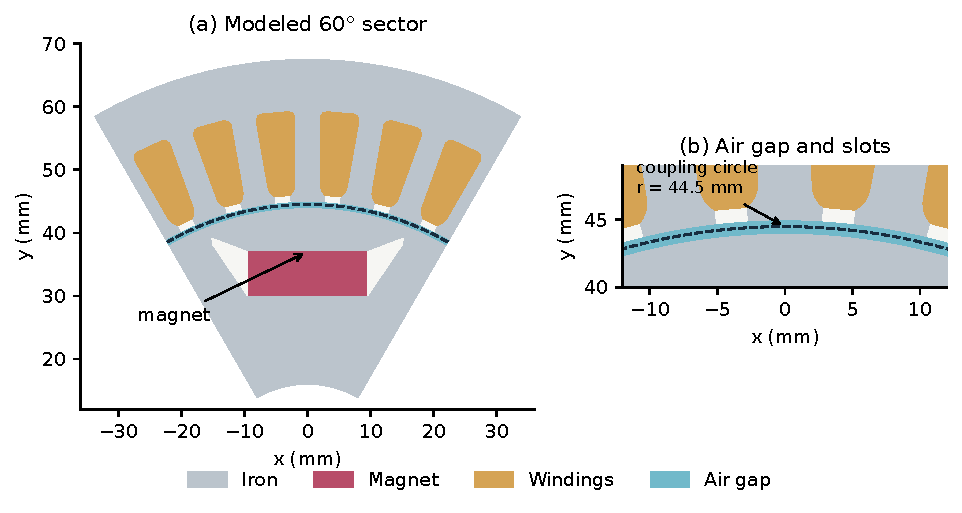
\includegraphics[width=\linewidth]{figures/geometry.pdf}
\caption{Initial-design geometry rendered directly from the committed
coarsest mesh. The dashed line is the rotor--stator coupling circle. The
right panel enlarges the gap and slot openings. Material boundaries are
shown without the element edges; the geometry is not an optimized result.}
\label{fig:geometry}
\end{figure}

The reconstruction uses the initial NURBS exports in the public snapshot.
Their control points are stored with weights already multiplied in, and
patch orientation must be accounted for when integrating areas. Two thin
rotor patches described as air slits in source comments receive iron under
the reference's material assignment; we follow that assignment. The
mesh generator preserves the winding groups separately, since their two
characteristic areas are approximately 36.29 and 31.22\,mm$^2$.

At mechanical angle $\beta$, phase currents are
\begin{equation}
 I_q(\beta)=a I_*\sin(\phi_0+3\beta+\delta_q),\qquad
 (\delta_U,\delta_V,\delta_W)=(0,-2\pi/3,2\pi/3),
 \label{eq:current}
\end{equation}
where $a\in\{0,0.5,1\}$, $I_*=9.677657374$\,A, and the electrical phase
offset $\phi_0=0$ for the initial design. Angles in
Eq.~\eqref{eq:current} are in radians. Each winding group carries current
density $J_g=12s_g I_q/|\Omega_g|$, with its own area and prescribed sign
$s_g\in\{-1,1\}$. Using a common area would change the current density
between groups by about 16\%. We compare 20 distinct mechanical angles,
$0^\circ,1^\circ,\ldots,19^\circ$, excluding the duplicated endpoint in
the source CSV. The reference's optimization grid contains the ten even
angles; both grids are retained in the artifacts.

\subsection{Nonlinear field equation}
The two-dimensional magnetic vector potential $A=A_z$ determines the
flux density $\mathbf B=(\partial_y A,-\partial_x A)$. Iron is described
by an isotropic reluctivity $\nu(|\mathbf B|^2)$, where reluctivity is
the inverse of permeability. For a test function $v$ that satisfies the
homogeneous constraints, the weak equation is
\begin{equation}
 \int_\Omega \nu(|\nabla A|^2)\nabla A\cdot\nabla v\dd\Omega
 =\int_\Omega J_z v\dd\Omega
  +\int_{\Omega_m}\mathbf M\cdot(\partial_y v,-\partial_x v)\dd\Omega.
 \label{eq:weak}
\end{equation}
Here $\mathbf M$ denotes the permanent-magnet source in
$\mathbf H=\nu\mathbf B-\mathbf M$. In the magnet,
$\mu_r=1.05$ and $B_r=1.4$\,T, so its source magnitude is
$H_c=B_r/(\mu_0\mu_r)$, not $B_r/\mu_0$. Its direction is $\pi/2$
in the rotor frame and rotates with the rotor. Air and windings have
$\mu_r=1$. The inner and outer circular boundaries have $A=0$.

We use continuous piecewise-linear triangles. With nodal vector $u$,
element gradients $g_i=\nabla\varphi_i$, $G=\nabla A$ and $s=G\cdot G$,
the residual derivative on one element is
\begin{equation}
 K^e_{ij}=|\Omega_e|\left[\nu(s)g_i\cdot g_j
       +2\nu'(s)(g_i\cdot G)(g_j\cdot G)\right].
 \label{eq:tangent}
\end{equation}
The second term is required when the material changes with field strength.
Newton steps use this consistent tangent, with damping and a stopping
reference independent of the initial guess. Constant potential offsets,
where allowed by the boundary conditions, do not change that reference.
The solver reports whether it stopped at the requested tolerance or an
estimated floating-point floor. All 500 solves in the recorded motor study
stopped at the requested tolerance.

The iron law uses 47 tabulated M27 $B$--$H$ points from 0 to 2.30\,T.
Monotonicity is imposed on $H(B)$, not on $\nu(B^2)=H(B)/B$.
In fact, the tabulated $H/B$ decreases between 0.05 and 0.10\,T.
The two material tangent eigenvalues must satisfy
\begin{equation}
 \nu>0,\qquad \nu+2s\nu'=\frac{\dd H}{\dd B}>0.
\end{equation}
The GEODE and reference interpolants agree to round-off between 0.05 and
2.25\,T. GEODE uses an odd cubic near zero and a continuous slope into the
vacuum-slope tail above 2.30\,T. The reference uses a low-field clamp and
a different last-knot slope. The maximum relative difference in
reluctivity near zero is 6.66\%; the last segment differs in $H$ by at
most $2.17\times10^{-4}$ relatively. We test the torque effect of the
low-field difference in Section~\ref{sec:sensitivity}.

\subsection{Rotation and torque}
At the modeled angles, the two circular traces have matching nodes after
rotation. The sliding interface identifies their potentials, including
the antiperiodic sign on sector wrap-around. Writing the full nodal vector
as $u=P\hat u+u_D$, the reduced residual and tangent are
$\hat R=P^T R(P\hat u+u_D)$ and $\hat K=P^T K P$.
The rotor geometry and magnet source rotate together; currents use the
same mechanical angle in Eq.~\eqref{eq:current}.

We average Maxwell stress over the air gap using the Arkkio expression
\begin{equation}
 T(\beta)=\frac{L}{\mu_0(r_2-r_1)}
  \int_{\Omega_{\rm gap}}r B_r B_\theta\dd\Omega,
 \qquad(r_1,r_2)=(44,45)\ {\rm mm}.
 \label{eq:torque}
\end{equation}
Positive torque acts counter-clockwise on the rotor. All torques in this
paper include axial length and refer to the modeled sector. We apply no
factor of six when comparing with the saved reference arrays, despite a
per-length label appearing in the reference evaluation plots.

The reference instead couples rotor and stator through eight angular
harmonic orders $3,9,\ldots,45$, represented by 16 sine/cosine modes.
It obtains torque from the derivative of that coupling with respect to
rotation. The interface and torque formulations therefore differ between
the two models even when the geometry and excitations agree.

\section{Verification and experiment design}
The implementation is checked before the motor comparison. With constant
material laws it agrees with the linear assembly to approximately
$2\times10^{-14}$ in potential. Central differences of the nonlinear
residual agree with the tangent action to below $10^{-9}$ at favorable
step sizes on the synthetic material tests. A manufactured solution gives
fitted spatial rates 1.002 in the $H^1$ seminorm and 2.007 in $L^2$.
For a saturated iron annulus carrying enclosed current $I$, the independent
radial field relation is $H(r)=I/(2\pi r)$, followed by inversion of the
material law. The M27 test reaches a mid-annulus relative field error of
$3.76\times10^{-4}$ on its finest mesh. These are verification results
for the forward model; they do not verify motor shape derivatives.

Sector tests compare the constrained solution with a full-machine solve,
check the reduced tangent by finite differences, and exercise positive,
negative and wrapped rotation steps. Clockwise and counter-clockwise
triangle orderings give equivalent magnet sources and fields. The motor
regression also detects changes in magnet strength, magnet direction,
phase ordering and rotation direction. Detailed logs accompany the code.

The motor study uses four meshes, L0--L3, with 3,153, 9,937, 36,083 and
139,268 nodes. The coupling circle has $120\,2^\ell$ segments at level
$\ell$, so integer-degree rotation is represented at every level.
Each level contains 60 baseline solves: three current levels and 20
angles. A solution at one angle initializes the next angle at the same
current. We report the mean and population standard deviation,
\begin{equation}
 \bar T=\frac1N\sum_{k=1}^N T_k,\qquad
 \sigma_T=\left[\frac1N\sum_{k=1}^N(T_k-\bar T)^2\right]^{1/2},
 \quad N=20.
\end{equation}
The standard deviation is the ripple metric used for the comparison.
At zero current it measures cogging, the torque variation caused by the
permanent magnets and slots without applied phase current.

For a scalar statistic $q$, the empirical L3 uncertainty interval is
\begin{equation}
 q_3\ \pm\ e_q,\qquad
 e_q=\max\{|q_2-q_1|,|q_3-q_2|\}.
 \label{eq:band}
\end{equation}
We use the same construction pointwise for waveforms. This interval is a
refinement diagnostic, not a proven error bound or a statistical confidence
interval. It does not cover reference-model error or angular quadrature
error. The loaded means change direction between the last two increments,
so a last-increment estimate alone would be particularly weak.

\section{Forward reproduction results}
\subsection{Mean agreement and ripple disagreement}
Table~\ref{tab:torque} separates the loaded mean from ripple. The mean is
0.15\% low at half current and 0.16\% low at full current. The respective
reference means lie 0.05\% and 0.07\% beyond the empirical L3 intervals,
so even the mean comparison is not agreement within that estimated
spatial error. The zero-current mean is close to zero and is reported
without a relative error.

\begin{table}[htbp]\centering\small
\caption{Finest-mesh comparison with saved reference output. Means and
standard deviations are in N\,m per sector; deviations use the reference
as denominator. Relative zero-current mean error is omitted.}
\label{tab:torque}
\setlength{\tabcolsep}{4pt}
\begin{tabular}{rrrrrrr}\toprule
$a$ & $\bar T_{\rm L3}$ & $\bar T_{\rm ref}$ & $\Delta\bar T$ (\%) & $\sigma_{\rm L3}$ & $\sigma_{\rm ref}$ & $\Delta\sigma$ (\%)\\\midrule
0 & 0.00001 & 0.00010 & --- & 0.00760 & 0.01071 & -29.1 \\
0.5 & 0.66106 & 0.66208 & -0.15 & 0.04279 & 0.03895 & +9.9 \\
1 & 1.44023 & 1.44248 & -0.16 & 0.08829 & 0.07935 & +11.3 \\
\bottomrule\end{tabular}

\end{table}

Ripple differs much more: 9.9\% and 11.3\% above the reference under load,
and 29.1\% below it at zero current. Figure~\ref{fig:waveforms} shows that
the discrepancy is a waveform difference, not simply a mean shift.
The reference lies outside the pointwise L3 intervals at 18, 18 and 17
of the 20 angles for zero, half and full current, respectively.

\begin{figure}[htbp]\centering
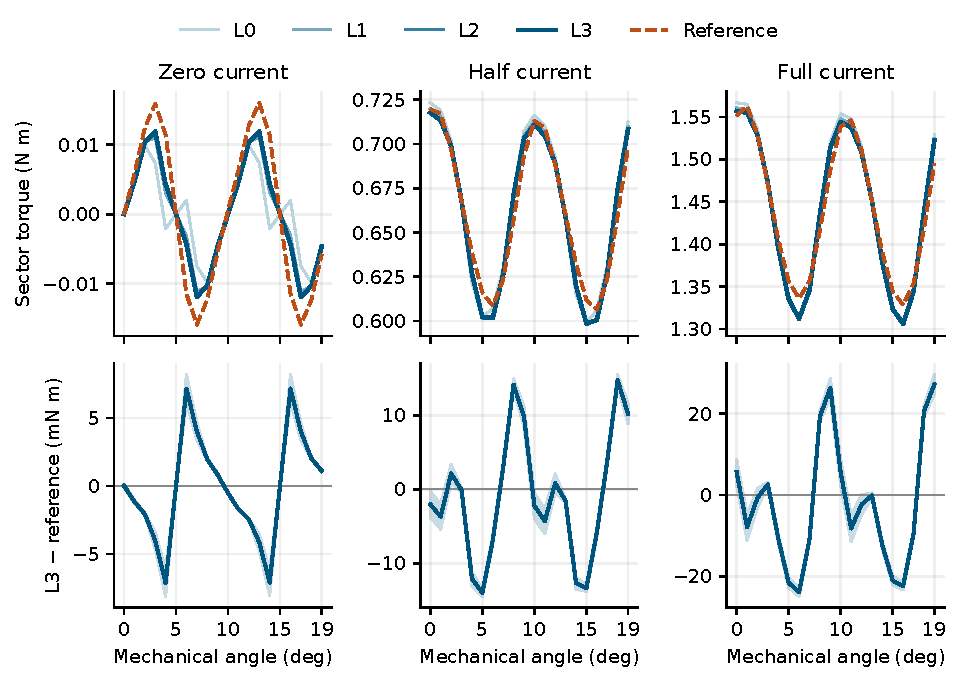
\includegraphics[width=\linewidth]{figures/waveforms.pdf}
\caption{Top: GEODE torque waveforms at four spatial resolutions and the
saved reference. Bottom: L3 minus reference, with the pointwise interval
from Eq.~\eqref{eq:band}. The three residual panels have independent
vertical scales. The shaded regions estimate spatial change in GEODE;
they do not quantify the reference's uncertainty.}
\label{fig:waveforms}\end{figure}

\subsection{Spatial refinement}
The maximum pointwise changes from L2 to L3 are $2.85\times10^{-4}$,
$5.60\times10^{-4}$ and $1.16\times10^{-3}$\,N\,m at the three
currents. They are smaller than the corresponding differences from the
reference, which reach 0.00715, 0.01471 and 0.02719\,N\,m.
Figure~\ref{fig:convergence} shows decreasing waveform increments while
the ripple discrepancies persist. The three ripple intervals are
$[0.00733,0.00786]$, $[0.04215,0.04342]$ and
$[0.08703,0.08955]$\,N\,m, each excluding its reference value.

\begin{figure}[htbp]\centering
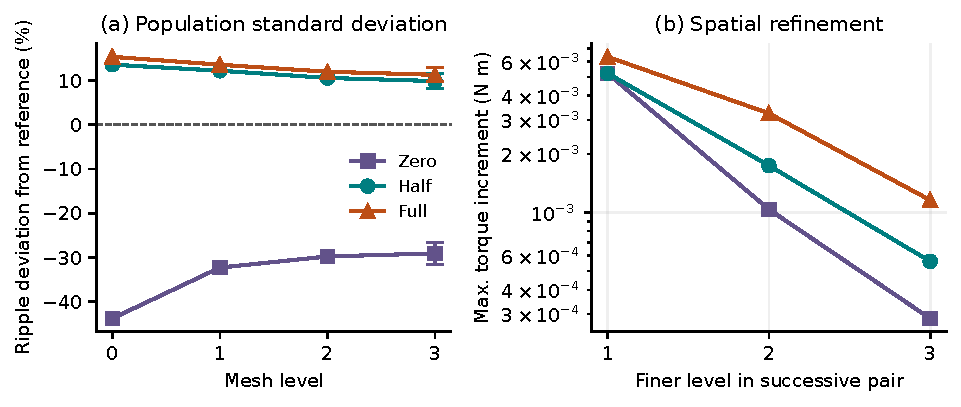
\includegraphics[width=\linewidth]{figures/convergence.pdf}
\caption{Spatial refinement of the initial motor. Left: relative ripple
deviation, with L3 error bars from Eq.~\eqref{eq:band}. Right: maximum
waveform difference between successive meshes. Neither plot establishes
continuum convergence of the independent reference calculation.}
\label{fig:convergence}\end{figure}

On the ten even angles used in the reference optimization, the L3 ripple
deviations are $-33.8\%$, $+9.5\%$ and $+10.7\%$ when compared with
the corresponding saved history values. The mismatch therefore persists
on that sampling grid. This comparison is not an angular convergence
study; denser and shifted angle grids remain necessary for design validation.

\subsection{Sensitivity and unresolved causes}\label{sec:sensitivity}
The controlled changes in Table~\ref{tab:sensitivity} are too small to
explain the observed waveform gap at the tested settings. The near-zero
material difference has particularly little effect on torque despite its
6.66\% local reluctivity difference. This is a measured sensitivity of
the initial design and does not establish insensitivity after optimization.

\begin{table}[htbp]\centering\small
\caption{Maximum absolute torque change relative to the baseline at the
same mesh level. Entries summarize the recorded angle/current subsets.}
\label{tab:sensitivity}
\begin{tabular}{p{.48\linewidth}ll}\toprule
Change & Levels & Max. $|\Delta T|$ (N\,m)\\\midrule
Reference low-field interpolation and clamp & L2, L3 & $2.1\times10^{-6}$\\
Relative Newton tolerance $10^{-12}$ vs $10^{-8}$ & L2; L3 full current & $7.3\times10^{-8}$\\
Exact winding areas vs mesh areas & L2 & $3.9\times10^{-4}$\\
Inner or outer half of the Arkkio band & L3 & $7.3\times10^{-5}$\\
\bottomrule\end{tabular}
\end{table}

Maxwell stress sampled on a single circle is less stable for the
piecewise-constant P1 field. At L3 its maximum differences from the
gap-averaged estimator range from about 0.0023 to 0.025\,N\,m across the
sampled radii and currents. That check does not independently validate
Arkkio torque to high precision; the half-band and spatial-refinement
results provide the present support for using the averaged estimator.

Two explanations remain open. First, the reference's eight harmonic
orders restrict what the rotor and stator exchange through the air gap.
Our conforming interface admits all modes resolved by the mesh. Filtering
the already-solved L3 gap field at order 45 changes the diagnostic cogging
standard deviation from about 0.0075 to 0.0184\,N\,m. This demonstrates
sensitivity to discarded modes, but it neither reproduces the reference
value nor supplies the field that a truncated-coupling solve would produce.
A matched harmonic-coupling solve is required to test the explanation.

Second, the saved reference uses degree-two isogeometric elements with
$3\times3$ subdivisions per patch. It is a reproduction target, not a
converged reference. Its own spatial and interface errors have not been
bounded. The reference's cogging symmetry residual is approximately
$5.5\times10^{-4}$\,N\,m, compared with less than
$4.8\times10^{-5}$\,N\,m in GEODE L3; symmetry alone cannot detect a
symmetric discretization error. The present evidence does not isolate
either coupling truncation or reference coarseness as the cause.

\subsection{Forward cost}
Table~\ref{tab:cost} reports recorded local, sequential release-build
timings on Apple Silicon. They describe the forward workload only, with
no matched timing of the reference implementation. Warm angle steps
typically require two or three Newton iterations; the initial L3 solves
require 12--14. The full sensitivity study records 500 solves and 3491 seconds of summed per-solve wall time. Hardware identification, thread limits
and repeat-run variation must be fixed before using timings for an
optimizer comparison.
\begin{table}[htbp]\centering
\caption{Recorded baseline forward cost. Median wall time is taken over
all 60 solves per mesh, including the three initial solves. Totals sum
per-solve wall time and exclude mesh generation and setup.}
\label{tab:cost}
\begin{tabular}{lrrr}\toprule
Mesh & Nodes & Median (s) & Sum, 60 solves (s)\\\midrule
L0 & 3,153 & 0.09 & 6.1 \\
L1 & 9,937 & 0.54 & 35.5 \\
L2 & 36,083 & 3.32 & 222.2 \\
L3 & 139,268 & 15.97 & 1072.8 \\
\bottomrule\end{tabular}

\end{table}

\section{Planned gradient and optimization comparison}\label{sec:planned}
The following experiment is prospective. The forward results above do
not include a motor shape derivative, an optimized geometry or a measured
optimization speedup. Resolving the ripple comparison, or quantifying
the remaining model difference, precedes those comparisons.

For a design vector $p$ and a converged reduced state $u(p)$ satisfying
$R(u,p)=0$, a scalar objective $F$ has total derivative
\begin{equation}
 \frac{\dd F}{\dd p}=F_p-\lambda^T R_p,\qquad
 R_u^T\lambda=F_u^T.
 \label{eq:adjoint}
\end{equation}
This identity follows by differentiating the residual and eliminating
$\dd u/\dd p$. Implementing it requires derivatives of geometry, loads,
material terms, constraints, interface motion and the actual torque
functional. Access to the converged tangent is one ingredient, not a
verification of all those derivatives. Directional finite-difference
step sweeps and Taylor remainder tests must be run at initial and perturbed
designs, with solver tolerances tightened enough to separate derivative
error from state error.

The proposed objective is the sum of squared ripple over zero, half and
full current, normalized by a fixed positive torque scale $T_*$:
\begin{equation}
 F(p)=\sum_{a\in\{0,0.5,1\}}
       \frac{\sigma_T(p,a)^2}{T_*^2}.
\end{equation}
This avoids division by the nearly zero mean cogging torque. Loaded mean
torque, minimum air gap, bridge thickness, magnet area and valid geometry
are constrained. The initial comparison fixes the outer envelope, axial
length and control policy. These choices define a controlled shape study;
they are not identical to every objective and parameter choice in the
reference optimization.

Two experiments must be kept separate. The first compares optimizers
within a common design space: exact gradients, finite differences as a
diagnostic, competitive derivative-free search, and calibrated physical
or waveform-surrogate models. The second expands a small engineering
parameter basis with shape controls while preserving the constraints and
validation target. Adding variables without a resolved performance gain
would not demonstrate useful shape freedom.

Costs begin with the first model or calibration evaluation and include
mesh updates, assembly, nonlinear solves, derivative assembly,
factorizations, constraints, line searches and surrogate training.
Each operating state and independent scalar adjoint output is counted;
there is no assumption that one backward solve handles all angles and
constraints. Methods share hardware, thread limits, initial designs,
targets and budgets, with valid reuse available to each method. Candidates
are checked on finer meshes, denser and shifted angles, tighter tolerances
and withheld currents. A method that fails to attain the target within its
budget is reported as such, rather than assigned a finite speedup ratio.

\section{Discussion and limitations}
The comparison demonstrates why forward validation should follow the
optimization objective. Agreement in mean torque supports the excitation
and normalization choices, but it is insufficient for an objective built
from angular variation. The ripple discrepancy is larger than the
observed GEODE spatial changes and the tested material and solver
sensitivities. Its cause still needs an experiment that changes the
coupling formulation while holding the other inputs fixed.

The proposed benchmark remains two-dimensional and magnetostatic. It
does not qualify thermal behavior, demagnetization, mechanical fatigue,
three-dimensional end effects, losses or a complete efficiency map.
The model is reconstructed from published computational artifacts; there
is no new experimental validation against a physical motor. Only the
initial design and the three specified current levels are evaluated here.
Neither the material sensitivity nor the refinement behavior can be
assumed to remain unchanged for a new geometry.

A simpler model is an essential control. At one fixed geometry, the
existing linear slotless fixture is represented by a three-coefficient
sinusoid with held-out-angle error near numerical precision
(Appendix~\ref{sec:slotless}). That observation does not test unseen
designs, but it shows why parameter count alone is a poor reason to
expect a gradient advantage. A competitive nonlinear reduced model might
also capture the design directions needed for the slotted motor.

\section{Conclusion}
A nonlinear finite-element reconstruction matches the published initial
motor's loaded mean torque within 0.16\%, while its ripple differs by
9.9--11.3\% under load and 29.1\% at zero current. Four spatial resolutions
and targeted sensitivity checks expose the discrepancy but do not resolve
its cause. The resulting model and evidence support the next comparison:
whether controlling interface and discretization error makes torque
ripple a stable target for shape optimization. The benefit of full-field
gradients remains an experimental question.

\section*{Code and data availability}
The evidence used here is fixed at GEODE commit
\href{https://github.com/rjwalters/geode-fem/tree/581ee7ad40c9646f43e0d6df3de7b5a87d06f798}{\texttt{581ee7ad}}.
The repository contains the
\href{https://github.com/rjwalters/geode-fem/tree/581ee7ad40c9646f43e0d6df3de7b5a87d06f798/benchmarks/motor_reference/forward}{raw motor runs and analysis},
\href{https://github.com/rjwalters/geode-fem/tree/581ee7ad40c9646f43e0d6df3de7b5a87d06f798/benchmarks/motor_reference/geometry}{geometry and mesh-generation scripts},
and \href{https://github.com/rjwalters/geode-fem/tree/581ee7ad40c9646f43e0d6df3de7b5a87d06f798/benchmarks/motor_nonlinear_m1}{solver verification logs}.
Reference data are extracted from the authors'
\href{https://github.com/MichaelWiesheu/ICEMsnapshot/tree/b145aaf4ab1a6424828bc941eaf172f48fa0d458}{ICEM snapshot at \texttt{b145aaf4}},
a later repository revision rather than a claim to the original conference
release. Source hashes, extraction checks and the upstream GPL-3.0 license
are retained. The paper package includes a manifest, copied figure inputs
and a regeneration script; it does not require rerunning FEM to rebuild
the figures. Recomputing the physical study requires the separately
documented mesh and solver commands.

\appendix
\section{Linear slotless screening control}\label{sec:slotless}
The stored slotless fixture has 24 distinct angles. Fitting
$T(\phi)=c_0+c_1\cos\phi+c_2\sin\phi$, with electrical angle $\phi=p\theta_r$ and pole-pair count $p$, on alternate angles and
evaluating on the other twelve gives normalized held-out RMSE
$3.08\times10^{-10}$ and maximum error $6.83\times10^{-10}$, using the
recorded analytic-amplitude normalization. This is a locked-rotor angle sweep,
not synchronous operating ripple. For a fixed linear field operator and
sinusoidal sources, the field lies in a small basis of source responses;
a quadratic torque functional can contain only the corresponding finite
set of harmonics. The particular fixture needs just the three fitted
coefficients. This is an angular interpolation test at one geometry,
not a shape-gradient test or evidence of generalization across designs.

\clearpage
\bibliographystyle{plainnat}
\bibliography{refs}
\end{document}
